%%%%%%%%%%%%%%%%%%%%%%%%%%%%%%%%%%%%%%%%%%%%%%%%%%%%%%%%%%%%%%%%%%%%%%%%%%%%%%%
\chapter{Movimento retilíneo uniforme (MRU) e uniformemente variado (MRUV)}
\label{Chap:ExpMRUMRUV}
%%%%%%%%%%%%%%%%%%%%%%%%%%%%%%%%%%%%%%%%%%%%%%%%%%%%%%%%%%%%%%%%%%%%%%%%%%%%%%%

\begin{fullwidth}\it
	Realizaremos dois experimentos distintos de forma a verificar as características do Movimento Retilíneo Uniforme -- MRU e do Movimento Retilíneo Uniformemente Variado -- MRUV. No primeiro caso, verificaremos a velocidade de uma esfera que se move em um fluido, sendo que ela atingirá uma velocidade terminal constante\footnote[][15mm]{Veremos o conceito de \emph{velocidade terminal} em detalhes na Experiência~\ref{Chap:ExpArrasto}.}. No segundo realizaremos um experimento de queda livre. Utilizaremos os conceitos de medidas, algarismos significativos, e gráficos.
\end{fullwidth}

%%%%%%%%%%%%%%%%%%%%%%%%%%%%%%%%%%%%%
\section[Gráficos]{Gráficos\footnote{O conteúdo dessa seção é um resumo do Capítulo~\ref{Chap:Graficos}.}}
%%%%%%%%%%%%%%%%%%%%%%%%%%%%%%%%%%%%%

Gráficos são ferramentas muito usadas para visualizar relações matemáticas entre uma função e seu argumento. Por exemplo, denominamos a função $f(x) = A + Bx$ como \emph{equação da reta}, pois seu gráfico é uma reta. Cada função tem um gráfico característico. 

Em experimentos de laboratório é comum procuramos estabelecer a relação entre duas grandezas. Para uma dessas variáveis escolhemos valores de acordo com nossa conveniência e a denominamos como \emph{variável independente}. Já a outra variável é mensurada e a denominamos como \emph{variável dependente}, pois seus valores dependem dos valores escolhidos para a variável independente. Denotamos a variáveis independente e dependente por $x$ e $y$, respectivamente. Nosso maior interesse, nesses casos, é justamente encontrar a função matemática $f$ que relaciona $x$ e $y$, ou seja, que nos dá $y$ \emph{em função de} $x$: $y = f(x)$.

Nos preocuparemos em estabelecer essa relação nos próximos experimentos. Hoje vamos discutir como elaborar um gráfico e o apresentar de forma clara.

%%%%%%%%%%%%%%%%%%%%%%%%%%%%%%%%%%%%%%
\subsection{Elaborando um gráfico}
%%%%%%%%%%%%%%%%%%%%%%%%%%%%%%%%%%%%%%

Hoje podemos fazer um gráfico rapidamente usando um programa de computador. No entanto, é interessante fazer alguns gráficos com papel milimetrado e lápis/caneta para sabermos o que tais programas estão fazendo. Além disso, existem vários tipos de gráficos, mas estamos interessados em um tipo específico, denominado em alguns programas como \emph{gráficos de dispersão}.

Um gráfico de dispersão consiste em dois eixos ---~um horizontal e outro vertical~--- em relação aos quais denotamos os valores de nossas medidas em pares ordenados. Se tomarmos as medidas da Tabela~\ref{Tab:TabelaDadosResfriamentoNoExp}, podemos fazer um gráfico como o da Figura~\ref{Fig:GraficoResfriamentoNoExp}.
\begin{margintable}[-5cm]
\centering
\begin{tabular}{ccccc}
\toprule
\multicolumn{2}{c}{Tubo 1} && \multicolumn{2}{c}{Tubo 2} \\
\cmidrule{1-2}\cmidrule{4-5}
$t$~(s) & $T~\tcdegree\textrm{C}$ & & $t$~(s) & $T~\tcdegree\textrm{C}$ \\
\midrule
\np{0}		& \np{98}	&& \np{0}		& \np{92} \\ 
\np{5,71}	& \np{93}	&& \np{8,27} 	& \np{87} \\
\np{17,79}	& \np{88}	&& \np{17,43}	& \np{82} \\
\np{34,50}	& \np{83}	&& \np{31,07}	& \np{77} \\
\np{61,63}	& \np{78}	&& \np{44,98}	& \np{72} \\
\np{83,96}	& \np{73}	&& \np{67,78}	& \np{67} \\
\np{109,09}	& \np{68}	&& \np{96,57}	& \np{62} \\
\np{130,78}	& \np{63}	&& \np{115,26}	& \np{57} \\
\np{149,09}	& \np{58}	&& \np{135,78}	& \np{52} \\
\np{184,21}	& \np{53}	&& \np{170,32}	& \np{47} \\
\np{217,09}	& \np{48}	&& \np{213,28}	& \np{42} \\
\np{261,28}	& \np{43}	&& \np{268,04}	& \np{37} \\
\np{315,90}	& \np{38}	&& \np{349,44}	& \np{32} \\
\np{373,35}	& \np{33}	&& \np{465,71}	& \np{27} \\
\np{470,55}	& \np{28}	&& \np{575,21}	& \np{24} \\
\np{504,21}	& \np{25} \\
\bottomrule
\end{tabular}
\vspace{1mm}
\caption{Dados para a temperatura de tubos metálicos em função do tempo para o processo de resfriamento convectivo.}
\label{Tab:TabelaDadosResfriamentoNoExp}
\end{margintable}

\begin{figure*}[!htb]\forceversofloat
\centering
\caption{Gráfico dos dados da Tabela~\ref{Tab:TabelaDadosResfriamentoNoExp}.}
\label{Fig:GraficoResfriamentoNoExp}
\begin{tikzpicture}[gnuplot]
%% generated with GNUPLOT 5.0p6 (Lua 5.3; terminal rev. 99, script rev. 100)
%% sex 30 ago 2019 10:39:24 -03
\path (0.000,0.000) rectangle (14.000,9.000);
\gpcolor{color=gp lt color border}
\gpsetlinetype{gp lt border}
\gpsetdashtype{gp dt solid}
\gpsetlinewidth{1.00}
\draw[gp path] (1.688,1.379)--(1.868,1.379);
\draw[gp path] (13.447,1.379)--(13.267,1.379);
\node[gp node right] at (1.504,1.379) {20,0};
\draw[gp path] (1.688,2.167)--(1.868,2.167);
\draw[gp path] (13.447,2.167)--(13.267,2.167);
\node[gp node right] at (1.504,2.167) {30,0};
\draw[gp path] (1.688,2.954)--(1.868,2.954);
\draw[gp path] (13.447,2.954)--(13.267,2.954);
\node[gp node right] at (1.504,2.954) {40,0};
\draw[gp path] (1.688,3.742)--(1.868,3.742);
\draw[gp path] (13.447,3.742)--(13.267,3.742);
\node[gp node right] at (1.504,3.742) {50,0};
\draw[gp path] (1.688,4.530)--(1.868,4.530);
\draw[gp path] (13.447,4.530)--(13.267,4.530);
\node[gp node right] at (1.504,4.530) {60,0};
\draw[gp path] (1.688,5.318)--(1.868,5.318);
\draw[gp path] (13.447,5.318)--(13.267,5.318);
\node[gp node right] at (1.504,5.318) {70,0};
\draw[gp path] (1.688,6.106)--(1.868,6.106);
\draw[gp path] (13.447,6.106)--(13.267,6.106);
\node[gp node right] at (1.504,6.106) {80,0};
\draw[gp path] (1.688,6.893)--(1.868,6.893);
\draw[gp path] (13.447,6.893)--(13.267,6.893);
\node[gp node right] at (1.504,6.893) {90,0};
\draw[gp path] (1.688,7.681)--(1.868,7.681);
\draw[gp path] (13.447,7.681)--(13.267,7.681);
\node[gp node right] at (1.504,7.681) {100,0};
\draw[gp path] (2.380,0.985)--(2.380,1.165);
\draw[gp path] (2.380,8.075)--(2.380,7.895);
\node[gp node center] at (2.380,0.677) {$0$};
\draw[gp path] (4.109,0.985)--(4.109,1.165);
\draw[gp path] (4.109,8.075)--(4.109,7.895);
\node[gp node center] at (4.109,0.677) {$100$};
\draw[gp path] (5.838,0.985)--(5.838,1.165);
\draw[gp path] (5.838,8.075)--(5.838,7.895);
\node[gp node center] at (5.838,0.677) {$200$};
\draw[gp path] (7.568,0.985)--(7.568,1.165);
\draw[gp path] (7.568,8.075)--(7.568,7.895);
\node[gp node center] at (7.568,0.677) {$300$};
\draw[gp path] (9.297,0.985)--(9.297,1.165);
\draw[gp path] (9.297,8.075)--(9.297,7.895);
\node[gp node center] at (9.297,0.677) {$400$};
\draw[gp path] (11.026,0.985)--(11.026,1.165);
\draw[gp path] (11.026,8.075)--(11.026,7.895);
\node[gp node center] at (11.026,0.677) {$500$};
\draw[gp path] (12.755,0.985)--(12.755,1.165);
\draw[gp path] (12.755,8.075)--(12.755,7.895);
\node[gp node center] at (12.755,0.677) {$600$};
\draw[gp path] (1.688,8.075)--(1.688,0.985)--(13.447,0.985)--(13.447,8.075)--cycle;
\node[gp node center,rotate=-270] at (0.246,4.530) {$T~(\tcdegree\textrm{C})$};
\node[gp node center] at (7.567,0.215) {$t$~(s)};
\node[gp node center] at (7.567,8.537) {Temperatura de um tubo sujeito a um resfriamento convectivo};
\node[gp node right] at (11.979,7.557) {Tubo N\textordmasculine~1};
\gpcolor{rgb color={0.000,0.000,0.000}}
\gpsetlinewidth{2.00}
\gpsetpointsize{4.00}
\gppoint{gp mark 5}{(2.380,7.524)}
\gppoint{gp mark 5}{(2.478,7.130)}
\gppoint{gp mark 5}{(2.687,6.736)}
\gppoint{gp mark 5}{(2.976,6.342)}
\gppoint{gp mark 5}{(3.445,5.948)}
\gppoint{gp mark 5}{(3.832,5.554)}
\gppoint{gp mark 5}{(4.266,5.160)}
\gppoint{gp mark 5}{(4.641,4.766)}
\gppoint{gp mark 5}{(4.958,4.372)}
\gppoint{gp mark 5}{(5.565,3.979)}
\gppoint{gp mark 5}{(6.134,3.585)}
\gppoint{gp mark 5}{(6.898,3.191)}
\gppoint{gp mark 5}{(7.842,2.797)}
\gppoint{gp mark 5}{(8.836,2.403)}
\gppoint{gp mark 5}{(10.517,2.009)}
\gppoint{gp mark 5}{(11.099,1.773)}
\gppoint{gp mark 5}{(12.621,7.557)}
\gpcolor{color=gp lt color border}
\node[gp node right] at (11.979,6.882) {Tubo N\textordmasculine~2};
\gpcolor{rgb color={0.000,0.000,0.000}}
\gppoint{gp mark 6}{(2.380,7.051)}
\gppoint{gp mark 6}{(2.523,6.657)}
\gppoint{gp mark 6}{(2.681,6.263)}
\gppoint{gp mark 6}{(2.917,5.869)}
\gppoint{gp mark 6}{(3.158,5.475)}
\gppoint{gp mark 6}{(3.552,5.081)}
\gppoint{gp mark 6}{(4.050,4.688)}
\gppoint{gp mark 6}{(4.373,4.294)}
\gppoint{gp mark 6}{(4.728,3.900)}
\gppoint{gp mark 6}{(5.325,3.506)}
\gppoint{gp mark 6}{(6.068,3.112)}
\gppoint{gp mark 6}{(7.015,2.718)}
\gppoint{gp mark 6}{(8.422,2.324)}
\gppoint{gp mark 6}{(10.433,1.930)}
\gppoint{gp mark 6}{(12.327,1.694)}
\gppoint{gp mark 6}{(12.621,6.882)}
\gpcolor{color=gp lt color border}
\gpsetlinewidth{1.00}
\draw[gp path] (1.688,8.075)--(1.688,0.985)--(13.447,0.985)--(13.447,8.075)--cycle;
%% coordinates of the plot area
\gpdefrectangularnode{gp plot 1}{\pgfpoint{1.688cm}{0.985cm}}{\pgfpoint{13.447cm}{8.075cm}}
\end{tikzpicture}
%% gnuplot variables

\end{figure*}

Neste gráfico podemos perceber que foram aplicados alguns princípios básicos para a elaboração de um gráfico adequado:
\begin{enumerate}
	\item O gráfico tem dois eixos devidamente nomeados com as variáveis que representam e com as unidades das medidas representadas.
	\item Ambos os eixos apresentam marcações com numerações que aparecem em \emph{intervalos regulares} ---~100 em 100 no eixo $x$ e a cada 10 no eixo $y$~---.
	\item O eixo $y$ foi ``cortado'', iniciando em um valor um pouco menor que 20. Isto é adequado pois não existem dados cujos valores da variável dependente sejam menores que \np[\tcdegree C]{20,0}.
	\item Os eixos começam e terminam de forma que toda a área disponível do gráfico é bem utilizada.
	\item O gráfico possui uma legenda indicando o que os pontos representam.
	\item Nenhum ponto fica excessivamente próximo dos eixos.
	\item Como há dois conjuntos de dados, temos uma diferenciação clara entre os pontos de cada conjunto.
\end{enumerate}


%%%%%%%%%%%%%%%%%%%%%%%%%%%%%%%%%%%%%%%%%%%%%%%%%%%%%
\subsection{Erros mais comuns ao elaborar um gráfico}
%%%%%%%%%%%%%%%%%%%%%%%%%%%%%%%%%%%%%%%%%%%%%%%%%%%%%

É difícil estabelecer um roteiro para elaborar um gráfico adequado, pois isso depende muito do que pretendemos mostar com ele. No entanto, existe uma série de \emph{erros comuns} ao elaborar um gráfico e que devem ser evitados:
\begin{description}
	\item[Não utilizar adequadamente a área do gráfico:] Muitas vezes nossos dados não iniciam em zero. Nesse caso devemos escolher um número próximo, porém inferior, ao primeiro valor que ocorre naquele eixo e iniciá-lo em tal número. Se, por exemplo, devemos marcar em um eixo os valores \np{107,25}, \np{115,12}, \np{129,90}, \np{138,22}, etc., uma boa escolha é iniciar o eixo em 100 e realizarmos as marcações no eixo a cada 10. Outra escolha adequada seria iniciar o eixo em 105 ---~porém, nesse caso, não marcamos o ``canto'' do gráfico\footnote{Foi o que escolhemos fazer no gráfico da Figura~\ref{Fig:GraficoResfriamentoNoExp}, cujo eixo $y$ começa em 15.} como 105~---. Realizamos a marcação em 110 e daí em diante a cada 10.
	\item[Não realizar marcações regulares nos eixos:] Marcações com ``espaçamento variável'' não devem ser realizadas. Utilizando os dados do item acima, poderíamos realizar marcações no eixo em \np{105}, \np{115}, \np{130} e \np{140}. Porém a distância entre essas marcações não é regular, o que dificulta a leitura do gráfico. Note que em um gráfico estamos interessados no comportamento qualitativo geral dos pontos, não nos valores específicos das variáveis que eles representam. Se desejarmos os valores, devemos buscá-los na tabela de dados.
	\item[Marcar os valores de $x$ e $y$ dos pontos experimentais:] Os valores de abscissas (valor no eixo $x$) e de ordenadas (valor no eixo $y$) dos pontos não devem aparecer nos eixos ordenados. Novamente, no gráfico não estamos interessados nos valores exatos das variáveis correspondentes aos pontos, mas sim no seu comportamento geral.
	\item[Linhas que ligam os pontos aos eixos:] Muitos alunos ligam os pontos aos eixos $x$ e $y$ usando linhas tracejadas. Não façam isso, mais uma vez, caso queiramos saber exatamente os valores nos eixos $x$ e $y$, podemos verificá-los na tabela de dados.
	\item[Linhas que ligam os pontos entre si:] Os pontos marcados a partir de dados experimentais nunca devem ser ligados entre si. Quando marcamos curvas ou retas em um gráfico, isso significa que temos conhecimento sobre todos os pontos que compõe aquela curva. Isso só pode ser razoável para os casos onde sabemos exatamente a função matemática que relaciona as variáveis $x$ e $y$, não para dados experimentais. Estes são verificados ``pontualmente'' e não podemos afirmar nada sobre o que obteríamos entre dois pontos quaisquer. Portanto, a reta que liga dois pontos experimentais não carrega informação alguma e não deve ser traçada.
    \item[Não diferenciar conjuntos de pontos diferentes:] É comum fazermos gráficos com mais que um conjunto de dados, com o intuito de compararmos seus comportamentos. Nesse caso, os conjuntos precisam ser diferenciados entre si. Para isso, basta utilizar símbolos diferentes para marcar os pontos, como quadrados, círculos, triângulos, etc., ou mesmo cores diferentes.
\end{description}

%%%%%%%%%%%%%%%%%%%%%%%%%%%%%%%%%%%%%%%%%%%%%%%%%%%%%%%%
\subsection{Elaborando um gráfico com papel milimetrado}
%%%%%%%%%%%%%%%%%%%%%%%%%%%%%%%%%%%%%%%%%%%%%%%%%%%%%%%%

Elaborar um gráfico em papel milimetrado é uma questão de observar as regras gerais para a elaboração de gráficos e usar regras de três. O procedimento para elaborar o gráfico consiste no seguinte:
\begin{enumerate}
	\item Verificar quais os valores mínimo $x_{\text{min}}$ e máximo $x_{\text{max}}$ para a variável do eixo $x$.
	\item Verificar quais os valores mínimo $y_{\text{min}}$ e máximo $y_{\text{max}}$ para a variável do eixo $y$.
	\item Verificar o tamanho do papel e desenhar os eixos \emph{dentro da área milimetrada} e não na borda. Em geral, deixa-se um centímetro entre a borda da área milimetrada e o eixo para que possamos fazer as escalas dos eixos.
	\item Decidimos os valores $x_i$, $x_f$, $y_i$, e $y_f$ em que os eixos $x$ e $y$ começam e terminam. Notem que devemos escolher valores tais que
	\begin{align}
	    x_i &< x_{\text{min}} & x_f &> x_{\text{max}} \\
	    y_i &< y_{\text{min}} & y_f &> y_{\text{max}}
	\end{align}
	\item Sabendo os valores $x_i$ e $x_f$ em que o eixo $x$ começa e termina, e que o eixo tem a medida $m$ no papel milimetrado, podemos marcar a ordenada do ponto $x_p$ a uma distância $d$ do início do eixo, onde $d$ é calculada como:
	\begin{equation}
		d = \frac{m(x_p-x_i)}{x_f-x_i}.
	\end{equation}
	Se, por exemplo, temos um conjunto de dados todo compreendido entre 30 e 110 e decidimos usar esses limites para fazer um gráfico de \np[cm]{25}, podemos encontrar a distância $d$ a partir do início do eixo em que devemos marcar o ponto $x_p=\np{47,2}$ através de
	\begin{align}
		d &= \frac{25\cdot(\np{47,2} - 30)}{110 - 30} \\
		  &= \numprint[cm]{5,375}.
	\end{align}
	\item O cálculo do item acima muitas vezes não é prático. Outra possibilidade é aproximarmos a escala: tomamos $x_f$, $x_i$ e $m$ e calculamos
		\begin{equation}
			f = \frac{x_f - x_i}{m}
		\end{equation}
		onde $f$ representa um ``fator de escala'' e após o calcularmos, o arredondamos para algum dos valores seguintes: 1, 2, 2,5, 4, 5 ou 10, ou qualquer múltiplo ou submúltiplo decimal desses valores (isto é, esses números multiplicados por 10 elevado a alguma potência inteira), sempre fazendo o arredondamento para cima. A partir desse valor arredondado $f'$, podemos calcular a distância $d$ entre o início do eixo e o ponto através de
		\begin{equation}
			d = \frac{x_p - x_i}{f'}.
		\end{equation}
\end{enumerate}

%%%%%%%%%%%%%%%%%%%%%%%%%%%%%%%%%%%%%%%%%%%%%%%%%%%%%%%%%%%%%%%%%%%%%%%%%%%%%%%
\section{Movimento retilíneo uniforme -- MRU}
%%%%%%%%%%%%%%%%%%%%%%%%%%%%%%%%%%%%%%%%%%%%%%%%%%%%%%%%%%%%%%%%%%%%%%%%%%%%%%%

Para um movimento unidimensional, a definição de velocidade média é dada por
\begin{equation}\label{Eq:DefVelMed}
    \mean{v} = \frac{\Delta x}{\Delta t}.
\end{equation}
%
Para o caso particular em que a velocidade é constante, para qualquer intervalo de tempo tomado, a razão acima resulta no mesmo valor. Nesse caso, dizemos que a velocidade é constante, ou \emph{uniforme}, e que a velocidade instantânea é idêntica à própria velocidade média:
\begin{equation}
    v \equiv \mean{v}.
\end{equation}

Explorando esse fato, podemos reescrever a Equação~\eqref{Eq:DefVelMed}, obtendo
\begin{align}
    \mean{v} &= \frac{\Delta x}{\Delta t} \\
    \Delta x &= \mean{v} \Delta t \\
    &= v \Delta t,
\end{align}
%
ou,
\begin{equation}
    x_f = x_i + v t,
\end{equation}
%
onde usamos $t_i \equiv 0$, $t_f \equiv t$. As variáveis $x_i$ e $x_f$ se referem aos valores de posição para os valores de $t_i$ e $t_f$ considerados, o que muitas vezes leva a notação
\begin{equation}
    x = x_0 + at.
\end{equation}
%
A expressão acima corresponde a uma função do tempo, uma vez que para cada valor dessa variável, temos um valor de posição distinto:
\begin{align}
    x(t) = x_0 + v t. \mathnote{Evolução temporal da posição para movimentos com velocidade constante.}
\end{align}

Comparando a equação acima com a equação de uma reta, verificamos que se fizermos um gráfico $x \times t$ ---~isto é, um gráfico de \emph{posição em função do tempo}, ou seja um gráfico onde o eixo horizontal representa o tempo e o vertical a posição~---, obteremos uma reta, como mostrado na Figura~\ref{Fig:GraficoRetaParaMovimentoComVelocidadeConstante}.

\begin{marginfigure}[2cm]
\centering
\begin{tikzpicture}
    \draw (0,0) -- (4,0) node[below left]{$t$};
    \draw (0,0) -- (0,3) node[below left]{$x$};
    
    \draw[thick] (-0.5, 0.74) -- node[above, near end, sloped]{$x(t)$} (4, 2.5);
\end{tikzpicture}
\caption{Para um movimento com velocidade constante, ao fazermos um gráfico $x \times t$ obtemos uma reta. Em particular, a figura acima representa a evolução da posição no tempo para um corpo cuja velocidade é positiva.\label{Fig:GraficoRetaParaMovimentoComVelocidadeConstante}}
\end{marginfigure}

%%%%%%%%%%%%%%%%%%%%%%%%%%%%%%%%%%%%%%%%%%%%%%%%%%%%%%%%%%%
\section{Movimento retilíneo uniformemente variado -- MRUV}
%%%%%%%%%%%%%%%%%%%%%%%%%%%%%%%%%%%%%%%%%%%%%%%%%%%%%%%%%%%

Para o movimento retilíneo com aceleração constante, podemos verificar de uma maneira análoga a descrita na seção anterior que a razão
\begin{equation}
    \mean{a} = \frac{\Delta v}{\Delta t}
\end{equation}
%
resulta sempre no mesmo valor, e a aceleração instantânea é igual ao próprio valor da aceleração média. Isso nos permite escrever
\begin{align}
    \mean{a} &= \frac{\Delta v}{\Delta t} \\
    \Delta v &= \mean{a} \Delta t \\
    v_f &= v_i + a \Delta t.
\end{align}
%
Note que a expressão acima indica uma variação uniforme na velocidade ---~isto é, uma variação linear/proporcional ao tempo transcorrido~---, por isso o movimento sujeito a uma aceleração constante é conhecido como \emph{uniformemente variado}. Em particular, se escolhermos $t_i = 0$, $t_f = t$, podemos escrever
\begin{equation}
    v = v_0 + at, \mathnote{Evolução temporal da velocidade para movimentos com aceleração constante.}
\end{equation}
%
onde $v_0$ representa a velocidade quando $t = 0$. De maneira análoga ao caso anterior, comparando a equação acima com a equação da reta, verificamos que ao fazer um gráfico $v \times t$ é dado por uma reta (Figura~\ref{Fig:GraficoRetaParaMovimentoComAceleracaoConstante}).
\begin{marginfigure}[3cm]
\centering
\begin{tikzpicture}
    \draw (0,0) -- (4,0) node[below left]{$t$};
    \draw (0,0) -- (0,3) node[below left]{$v$};
    
    \draw[thick] (-0.5, 0.74) -- node[above, near end, sloped]{$v(t)$} (4, 2.5);
\end{tikzpicture}
\caption{Para um movimento com aceleração constante, ao fazermos um gráfico $v \times t$ obtemos uma reta. Em particular, a figura acima representa a evolução da posição no tempo para um corpo cuja aceleração é positiva.\label{Fig:GraficoRetaParaMovimentoComAceleracaoConstante}}
\end{marginfigure}

Em um gráfico da velocidade em função do tempo para uma função $v(t)$ qualquer, podemos determinar o deslocamento sofrido pelo corpo cuja velocidade é descrita por tal função, em um dado intervalo de tempo, através da área delimitada pela curva $v(t)$, pelo eixo horizontal $t$, e pelas retas verticais que passam pelos valores $t_i$ e $t_f$ que delimitar o intervalo de tempo. Para o caso de um movimento que ocorre com velocidade constante, temos a área destacada na Figura~\ref{Fig:Graf_area_acel_const}. Podemos determinar uma expressão para o deslocamento ao dividir tal área em um retângulo e um triângulo, de onde obtemos
A área $A_1$ é dada por
\begin{align}
	A_1 &= v_i \Delta t \\
	A_2 &= \frac{(v_f - v_i)\Delta t}{2}.
\end{align}

\begin{marginfigure}[1cm]
\centering
\begin{tikzpicture}[>=Stealth, extended line/.style={shorten >=-#1,shorten <=-#1},
 extended line/.default=3mm]] % talvez fosse melhor amplicar com scale=1.5
    % Draw axes: acho que o |- é pra desenhar um "canto", um L
    \draw [<->,thick] (0,3) node (yaxis) [below left] {$v$}
        |- (4.3,0) node (xaxis) [below left] {$t$};
    % Desenhar função:
    \draw[smooth,name path=plot,samples=1000,domain=0:2.8]
    plot(\x,{0.7 + 0.5 * \x});

    \coordinate (a) at (0.5,0);
    \coordinate (b) at (2.5,0);
    \path[name path=froma](a)--+(0,3);
    \path[name path=fromb](b)--+(0,3);

 	\draw[dashed, name intersections={of=froma and plot}](a) node[below]{$t_i$} --(intersection-1) coordinate (plot-a-intersection)--(0,0|-intersection-1) node[left]{$v_i$};
 	\draw[dashed, name intersections={of=fromb and plot}](b) node[below]{$t_f$} --(intersection-1) coordinate (plot-b-intersection)--(0,0|-intersection-1) node[left]{$v_f$};

    \fill [pattern=north west lines, pattern color=gray, domain=0.5:2.5, variable=\x]
     	  (0.5, 0)
    	  -- plot ({\x}, {0.7 + 0.5 * \x})
          -- (2.5, 0)
          -- cycle;

	\draw[dashed](plot-a-intersection) -- +(2,0);

	\node[circle, fill=white, scale=0.7] (anode) at (1.5,0.5) {$A_1$};
	\node[circle, fill=white, scale=0.7] (anode) at (2,1.3) {$A_2$};

\end{tikzpicture}
\caption{Para o caso de aceleração constante, podemos calcular a área a dividindo em um retângulo e um triângulo.\label{Fig:Graf_area_acel_const}}
\end{marginfigure}

\noindent{}Logo,
\begin{equation}\label{Eq:DeltaComoSomaAreas}
  \Delta x = v_i\Delta t + \frac{(v_f - v_i)\Delta t}{2}.
\end{equation}
%
Utilizando a equação $v_f = v_i + at$, e fazendo ainda $t_i = 0$ e $t_f = t$, temos
\begin{equation}
  \Delta x = v_i t + \frac{(v_i + at - v_i) t}{2}
\end{equation}
%
e, finalmente,
\begin{equation}\label{Eq:XX0V0TAT22}
  x_f = x_i + v_i t +\frac{at^2}{2}.\mathnote{Evolução temporal da posição para aceleração constante.}
\end{equation}

\begin{marginfigure}[3cm]
\centering
\begin{tikzpicture}[>=Stealth, extended line/.style={shorten >=-#1,shorten <=-#1},
 extended line/.default=3mm]] % talvez fosse melhor amplicar com scale=1.5
    % Draw axes: acho que o |- é pra desenhar um "canto", um L
    \draw [<->,thick] (0,3) node (yaxis) [below left] {$x$}
        |- (4.3,0) node (xaxis) [below left] {$t$};
    % Desenhar função:
    \draw[smooth,name path=plot,samples=1000,domain=0:2.8]
    plot(\x,{0.6 - 0.5 * \x + 0.4 *\x*\x});
    
\end{tikzpicture}
\caption{Gráfico da função $x(t)$ para o caso $a > 0$. Note que a velocidade em $t = 0$ é negativa, por isso $x$ diminui com o passar do tempo até chegar a um valor mínimo para só então passar a aumentar.\label{Fig:Graf_Eq_Evol_Pos_a_const}}
\end{marginfigure}

Se escrevermos a expressão acima como uma função, temos
\begin{equation}
    x(t) = x_0 + v_0 t + \frac{at^2}{2},
\end{equation}
%
onde $x_0$ e $v_0$ representam a posição e a velocidade, respectivamente, para $t = 0$. Ao fazermos um gráfico $x \times t$ da posição em função do tempo, obtemos uma \emph{parábola} (Figura~\ref{Fig:Graf_Eq_Evol_Pos_a_const}). Isso se deve ao fato de que a expressão acima segue a forma
\begin{equation}
    y = A x^2 + Bx + C,
\end{equation}
%
que define a parábola.

%%%%%%%%%%%%%%%%%%%%%%%%%%%%%%%%%%%%%%%%%%%%%%%%%%%%%%%%%%%%%%%%%%%%%%%%%%%%%%%%%%%%
\section{Experimento: Determinação da evolução temporal da posição no MRU e no MRUV}
%%%%%%%%%%%%%%%%%%%%%%%%%%%%%%%%%%%%%%%%%%%%%%%%%%%%%%%%%%%%%%%%%%%%%%%%%%%%%%%%%%%%

Como exemplos de movimento retilíneo uniforme e de movimento retilíneo uniformemente variado, vamos realizar dois experimentos simples.

O primeiro consistirá em verificar o movimento de uma esfera metálica dentro de um tubo cilíndrico transparente, sendo que o volume interno do tubo está preenchido por um fluido viscoso e transparente. O tubo está afixado a um plano inclinado articulado, de forma que podemos variar o ângulo de inclinação. Devido à força de arrasto oferecida pelo fluido, a esfera se move a uma velocidade constante. Vamos coletar dados experimentais para duas posições de referência, bem como para o tempo necessário para que a distância entre tais posições seja transcorrida pela esfera metálica. Tais dados serão utilizados para a elaboração de um gráfico, além de determinarmos a velocidade da esfera.

No segundo caso, vamos verificar o movimento de uma esfera metálica ferromagnética em queda livre, sujeita à aceleração da gravidade. Vamos coletar dados para a posição inicial e final de dois sensores óticos, além do tempo necessário para que uma esfera em queda livre transcorra a distância entre eles. A esfera é inicialmente suspensa devido a ação de um eletroímã e, após ser solta, atravessa os dois sensores óticos, sendo que o primeiro dispara um cronômetro e o segundo o para. Através dos dados, vamos elaborar um gráfico e também determinaremos a aceleração da gravidade.

%%%%%%%%%%%%%%%%%%%%%%
\subsection{Objetivos}
%%%%%%%%%%%%%%%%%%%%%%

\begin{enumerate}
     \item Verificar as características do Movimento Retilíneo Uniforme -- MRU através do gráfico do tempo em função do deslocamento.
     \item Verificar as características do Movimento Retilíneo Uniformemente Variado -- MRUV através do gráfico do tempo em função do deslocamento.
     \item Calcular a velocidade do MRU;
     \item Determinar a aceleração da gravidade no MRUV;
\end{enumerate}

%%%%%%%%%%%%%%%%%%%%%%%%%%%%%%%%%%%%%%%%%%%%%%%%%%%%%%%%%%%%%%%%%%%%%%%%%%%%%%%
\section{Material Necessário}
%%%%%%%%%%%%%%%%%%%%%%%%%%%%%%%%%%%%%%%%%%%%%%%%%%%%%%%%%%%%%%%%%%%%%%%%%%%%%%%

\begin{itemize}
	\item Plano inclinado articulado com tubo lateral preenchido com fluido e dotado de esfera metálica ferromagnética livre para se mover dentro do tubo;
	\item Aparato de queda livre dotado de sensores óticos de movimento e de cronômetro eletrônico;
	\item Cronômetro manual;
	\item Régua (\np[m]{1,00});
	\item Ímã permanente.
\end{itemize}

%%%%%%%%%%%%%%%%%%%%%%%%%%%%%%%%%%%%%%%%%%%%%%%%%%%%%%%%%%%%%%%%%%%%%%%%%%%%%%%
\subsection{Procedimento Experimental}
%%%%%%%%%%%%%%%%%%%%%%%%%%%%%%%%%%%%%%%%%%%%%%%%%%%%%%%%%%%%%%%%%%%%%%%%%%%%%%%

\begin{marginfigure}
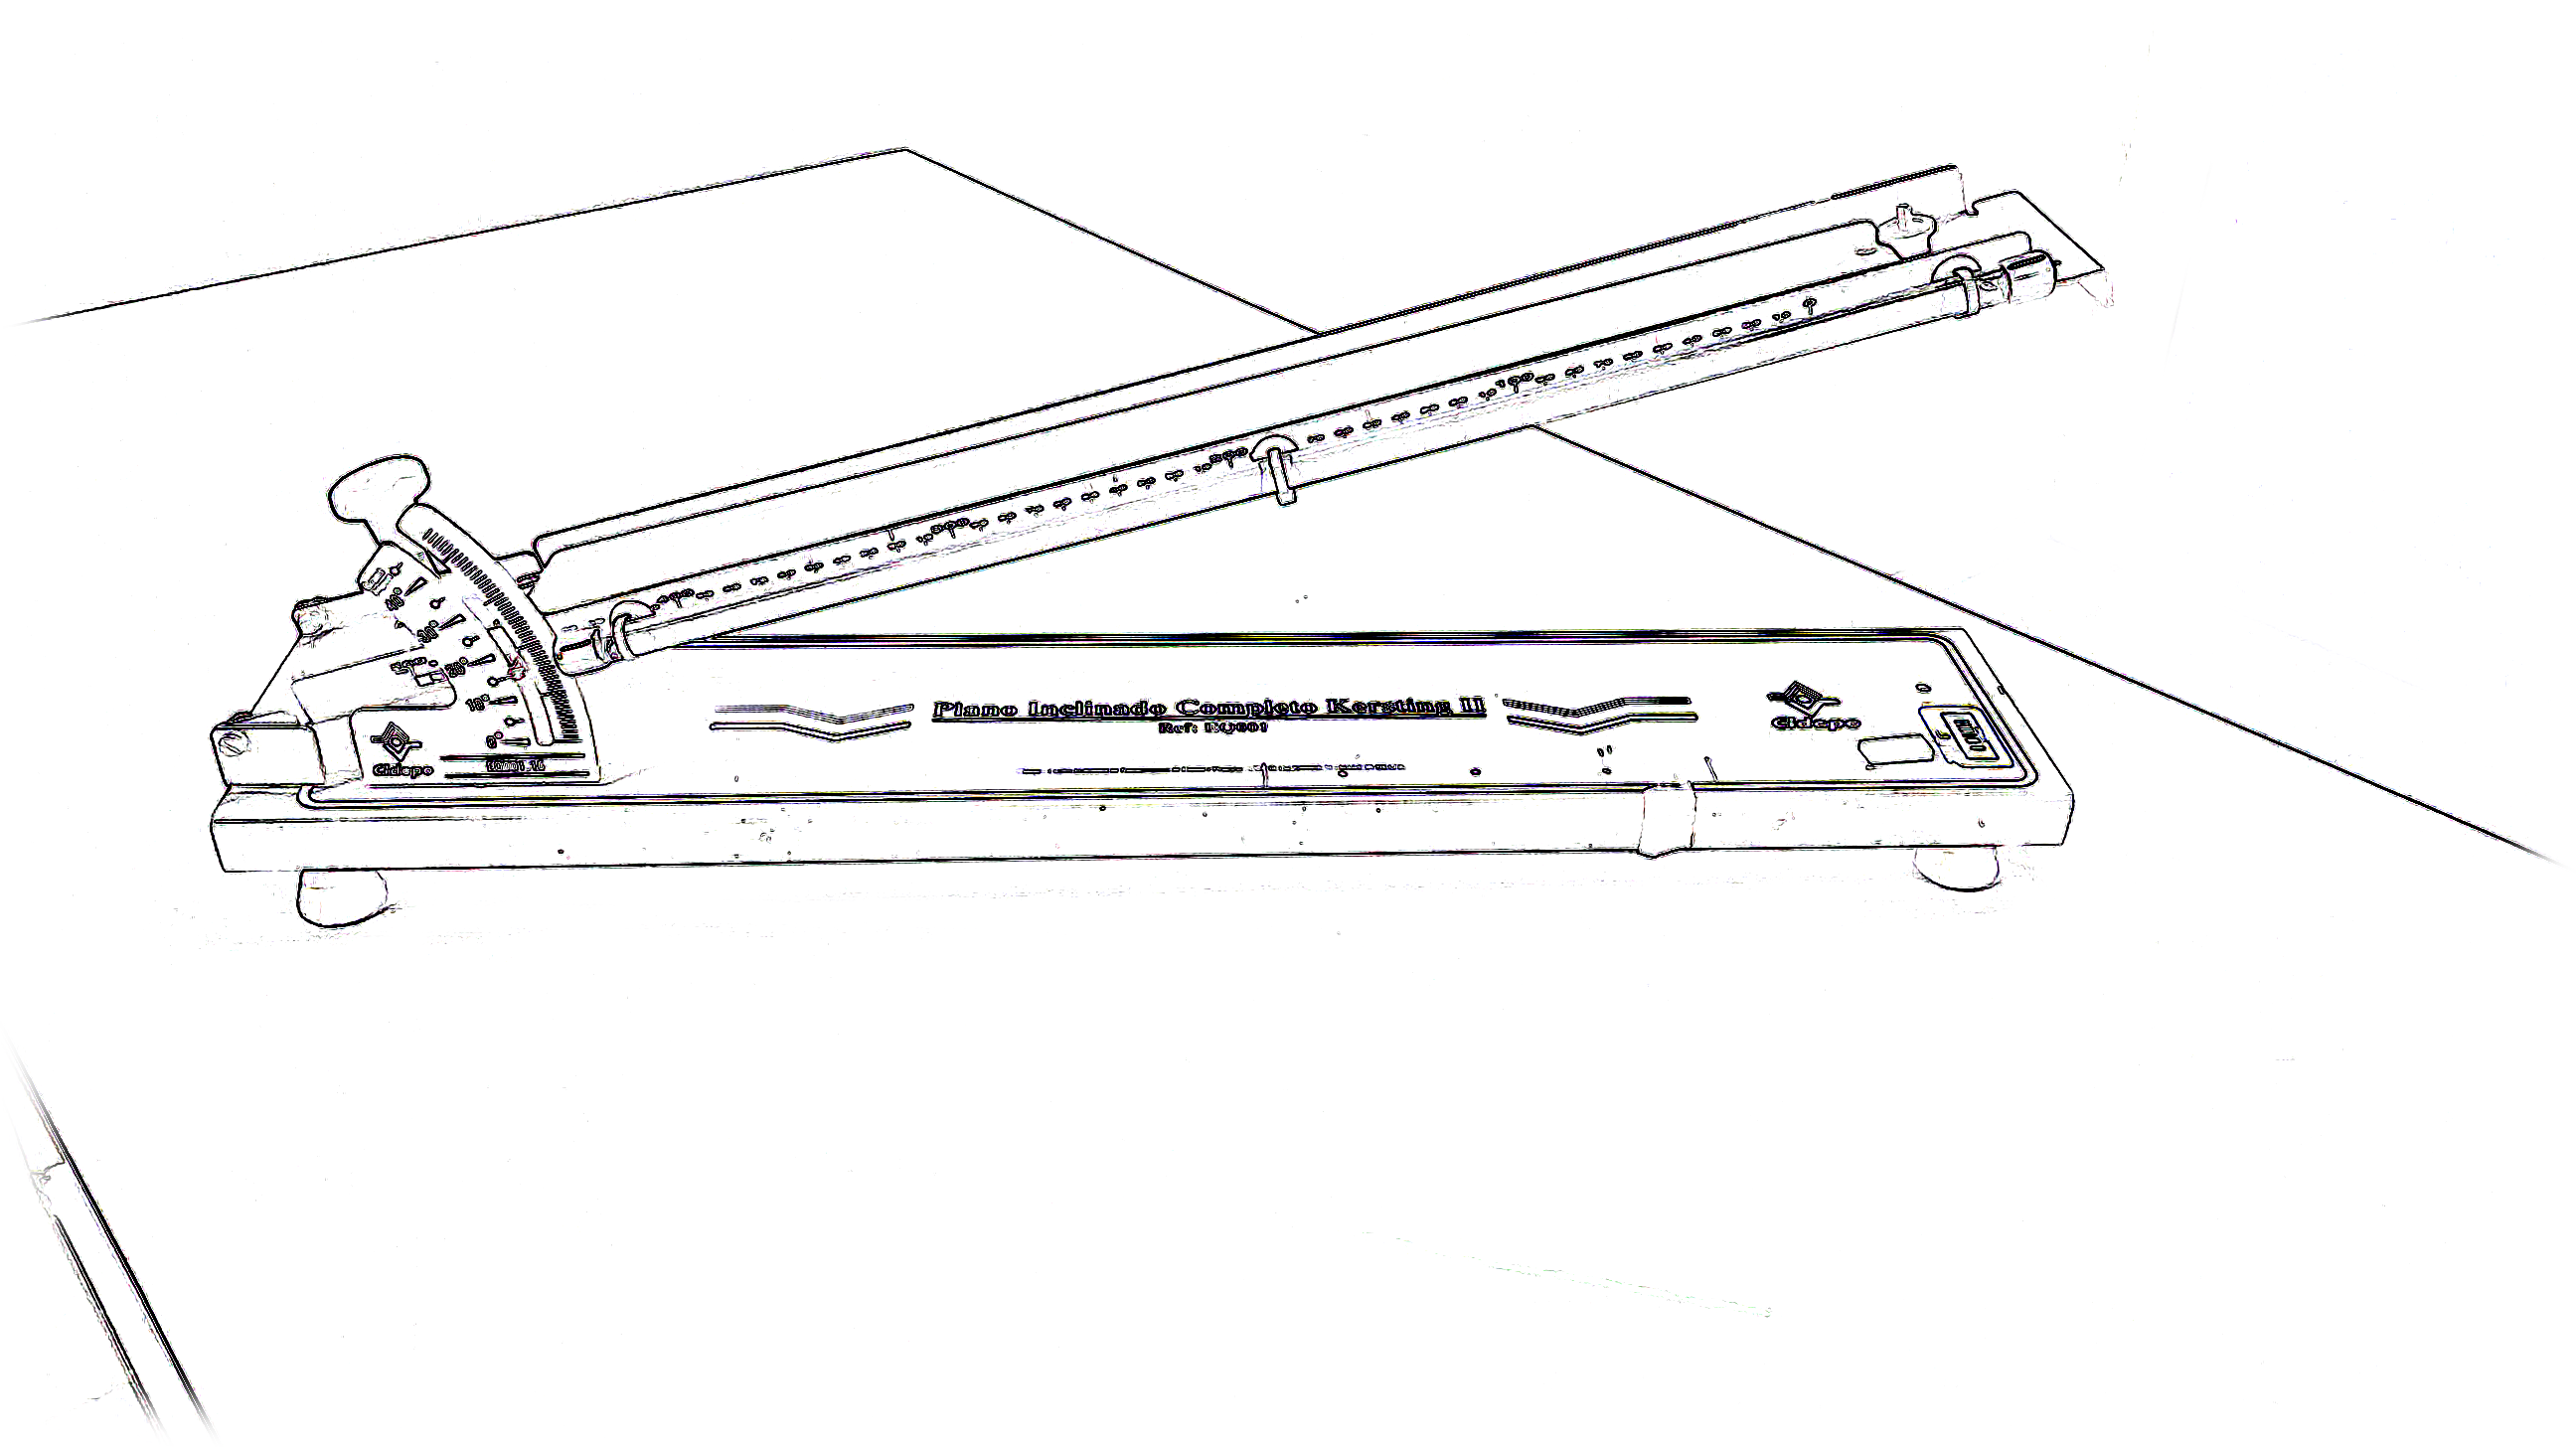
\includegraphics[width=\linewidth]{Ilustrations/Arrasto.png}
\caption{Plano inclinado com tubo preenchido com um fluido viscoso.}
\end{marginfigure}

%%%%%%%%%%%%%%%%%%%%%%%%%%%%%%%%%%%%%%%%%%%%%%%%%%%%%%%%%%%%%%%%%%%%%
\paragraph{MRU -- Deslocamento da esfera no tubo com fluido viscoso:}
%%%%%%%%%%%%%%%%%%%%%%%%%%%%%%%%%%%%%%%%%%%%%%%%%%%%%%%%%%%%%%%%%%%%%

\begin{enumerate}
	\item Ajuste o plano inclinado para um ângulo de \np[\tcdegree]{20,0};
	\item Com um imã, atraia a esfera para a parte superior antes da posição \np[cm]{0,0};\label{Item:Coleta1}
	\item Zere o cronômetro;
	\item Solte a esfera e inicie o cronômetro quando a ela passar pela posição \np[cm]{0,0}. Pare o cronômetro quando a ela passar pela posição final \np[cm]{10,0}. Anote os valores da posição inicial, final, e o tempo registrado pelo cronômetro na Tabela~\ref{DadosMRU};
	\item Repita este procedimento para os seguintes valores de posição final: \np[cm]{15}, \np[cm]{20}, \np[cm]{25}, \np[cm]{30}, \np[cm]{35}, \np[cm]{40}. A cada medida, anote os valores da posição inicial, final, e o tempo registrado pelo cronômetro na Tabela~\ref{DadosMRU};\label{Item:ColetaUltima}
	\item Ajuste o plano inclinado para um ângulo de \degree{40};
	\item Repita os procedimentos do itens \ref{Item:Coleta1} a \ref{Item:ColetaUltima} e anote os dados obtidos na Tabela~\ref{DadosMRU2}.
\end{enumerate}

%%%%%%%%%%%%%%%%%%%%%%%%%%%%%%%%%%%%%%%%%%%%
\paragraph{MRUV -- Queda livre:}
%%%%%%%%%%%%%%%%%%%%%%%%%%%%%%%%%%%%%%%%%%%%

\begin{enumerate}
    \item Ligue o cronômetro através do botão na parte de trás do aparelho;
    \item Certifique-se de que o cronômetro esteja operando na função \texttt{F1} e que o potenciômetro na parte de trás esteja no menor valor de potência que é capaz de prender a esfera;
    \item Ligue o eletroímã através do disjuntor;
	\item Prenda a esfera no eletroímã;
	\item Posicione o sensor superior de forma que ele fique muito próximo de ativar o cronômetro (erga o sensor com o cronômetro ligado e, quando o sensor ativar, desça um pouco, afixando sua posição). Verifique a posição\footnote{Use a escala do próprio suporte vertical do aparato.} inicial do sensor e a anote na Tabela~\ref{DadosMRUV};
	\item Posicione o sensor inferior \np[cm]{5,00} abaixo do primeiro e anote o valor de sua posição\footnote{Novamente, use a escala do próprio suporte vertical do aparato.} na Tabela~\ref{DadosMRUV};
	\item Certifique-se de que o cronômetro esteja zerado;
	\item Desligue o eletroímã e anote o valor do tempo registrado pelo cronômetro para a passagem da esfera na Tabela~\ref{DadosMRUV};
	\item Repita a medida de tempo mais duas vezes, anotando os resultados;
	\item Desloque o sensor inferior mais \np[cm]{5,0} anotando o valor de sua nova posição na Tabela~\ref{DadosMRUV};\label{ItemLoopMRUV}
	\item Ligue o eletroímã através do disjuntor e prenda nele a esfera;
	\item Zere o cronômetro;
	\item Desligue o eletroímã e anote o valor do tempo registrado pelo cronômetro para a passagem da esfera na Tabela~\ref{DadosMRUV}, repetindo a medida mais duas vezes e anotando os resultados;
	\item Repita os itens a partir do item \ref{ItemLoopMRUV} até completar a Tabela~\ref{DadosMRUV} ou não ser mais possível deslocar o sensor inferior.
\end{enumerate}

%%%%%%%%%%%%%%%%%%%%%%%%%%%%%%%%%%%%%%%%%%%%%%%%%%%%%%%%%%%%%%%%%%%%%%%%%%%%%%%
%%%%%%%%%%%%%%%%%%%%%%%%%%%%%%%%%%%%%%%%%%%%%%%%%%%%%%%%%%%%%%%%%%%%%%%%%%%%%%%
%%%%%%%%%%%%%%%%%%%%%%%%%%%%%%%%%%%%%%%%%%%%%%%%%%%%%%%%%%%%%%%%%%%%%%%%%%%%%%%
%%%%%%%%%%%%%%%%%%%%%%%%%%%%%%%%%%%%%%%%%%%%%%%%%%%%%%%%%%%%%%%%%%%%%%%%%%%%%%%
\cleardoublepage

\noindent{}{\huge\textit{Movimento retilíneo uniforme (MRU) e uniformemente variado (MRUV)}}

\vspace{15mm}

\begin{fullwidth}
\noindent{}\makebox[0.6\linewidth]{Turma:\enspace\hrulefill}\makebox[0.4\textwidth]{  Data:\enspace\hrulefill}
\vspace{5mm}

\noindent{}\makebox[0.6\linewidth]{Aluno(a):\enspace\hrulefill}\makebox[0.4\textwidth]{  Matrícula:\enspace\hrulefill}

\noindent{}\makebox[0.6\linewidth]{Aluno(a):\enspace\hrulefill}\makebox[0.4\textwidth]{  Matrícula:\enspace\hrulefill}

\noindent{}\makebox[0.6\linewidth]{Aluno(a):\enspace\hrulefill}\makebox[0.4\textwidth]{  Matrícula:\enspace\hrulefill}

\noindent{}\makebox[0.6\linewidth]{Aluno(a):\enspace\hrulefill}\makebox[0.4\textwidth]{  Matrícula:\enspace\hrulefill}

\noindent{}\makebox[0.6\linewidth]{Aluno(a):\enspace\hrulefill}\makebox[0.4\textwidth]{  Matrícula:\enspace\hrulefill}
\end{fullwidth}

\vspace{5mm}

%%%%%%%%%%%%%%%%%%%%%%%%%%%%%%%%%%%%%%%%%%%%%%%%%%%%%%%%%%%%%%%%%%%%%%%%%%%%%%%
\section{Questionário}
%%%%%%%%%%%%%%%%%%%%%%%%%%%%%%%%%%%%%%%%%%%%%%%%%%%%%%%%%%%%%%%%%%%%%%%%%%%%%%%

\begin{question}[type={exam}]{1}
Apresente os resultados de maneira clara e organizada. Mostre os cálculos requisitados de maneira clara e sucinta, evidenciando o raciocínio desenvolvido.
\end{question}

\begin{question}[type={exam}]{2}
Preencha as colunas de dados experimentais das tabelas com o número adequado de algarismos significativos e unidades.
\end{question}

\begin{question}[type={exam}]{1.5}
Calcule o deslocamento $\Delta x$, o tempo médio $\mean{t}$, e a velocidade para dos dados das Tabelas~\ref{DadosMRU} e~\ref{DadosMRU2}. Observe o número adequado de algarismos significativos e unidades.
\end{question}

\begin{question}[type={exam}]{2}
Para os dados das Tabelas~\ref{DadosMRU} e~\ref{DadosMRU2}, elabore em papel milimetrado um gráfico $x \times \mean{t}$, ou seja, da \emph{distância} percorrida pela esfera contida no tubo do plano inclinado em função do valor médio de \emph{tempo} (isto é, com a distância no eixo $y$ e o tempo no eixo $x$).\footnote{Note que a variável independente em nosso experimento é o deslocamento, sendo que deveríamos colocá-la no eixo horizontal, enquanto o tempo é nossa variável dependente e deveria estar no eixo vertical. Para fins didáticos, no entanto, vamos inverter essa relação para obter um gráfico mais usual.} Note que os dois conjuntos de dados devem ser representados no mesmo gráfico.
\end{question}

\begin{question}[type={exam}]{1.5}
Calcule o o deslocamento $\Delta x$ e o tempo médio $\mean{t}$ para os dados da Tabela~\ref{DadosMRUV}. Considerando que a velocidade inicial da esfera no movimento de queda livre é nula, calcule a aceleração da gravidade. Observe o número adequado de algarismos significativos e unidades.
\end{question}

\begin{question}[type={exam}]{2}
Para os dados da Tabela~\ref{DadosMRUV}, elabore em papel milimetrado um gráfico $x \times \mean{t}$, ou seja, um gráfico da \emph{distância} percorrida pela esfera em queda livre em função dos valores médios de \emph{tempo}.\footnote{Novamente, a variável independente é o deslocamento e deveria estar no eixo horizontal, enquanto o tempo é a variável dependente e deveria estar no eixo vertical. Para fins didáticos, vamos inverter essa relação para obter um gráfico mais usual.}
\end{question}
\vfill
%%%%%%%%%%%%%%%%%%%%%%%%%%%%%%%%%%%%%%%%%%%%%%%%%%%%%%%%%%%%%%%%%%%%%%%%%%%%%%%
\pagebreak
\section{Tabelas}
%%%%%%%%%%%%%%%%%%%%%%%%%%%%%%%%%%%%%%%%%%%%%%%%%%%%%%%%%%%%%%%%%%%%%%%%%%%%%%%

\begin{table*}[!ht]
\centering
\begin{tabular}{lp{25mm}p{25mm}p{25mm}p{25mm}p{25mm}l}
\toprule
	&\multicolumn{4}{l}{\textbf{Dados Experimentais}} \\
	\cmidrule{2-6}
	& $x_0$ & $x_f$ & $t_1$ & $t_2$ & $t_3$ & \\
	\cmidrule{2-6}
	& \cellcolor[gray]{0.89} & \cellcolor[gray]{0.92} & \cellcolor[gray]{0.89} & \cellcolor[gray]{0.92} & \cellcolor[gray]{0.89} \\
	& \cellcolor[gray]{0.95} & \cellcolor[gray]{0.97} & \cellcolor[gray]{0.95} & \cellcolor[gray]{0.97} & \cellcolor[gray]{0.95} \\
	& \cellcolor[gray]{0.89} & \cellcolor[gray]{0.92} & \cellcolor[gray]{0.89} & \cellcolor[gray]{0.92} & \cellcolor[gray]{0.89} \\
	& \cellcolor[gray]{0.95} & \cellcolor[gray]{0.97} & \cellcolor[gray]{0.95} & \cellcolor[gray]{0.97} & \cellcolor[gray]{0.95} \\
	& \cellcolor[gray]{0.89} & \cellcolor[gray]{0.92} & \cellcolor[gray]{0.89} & \cellcolor[gray]{0.92} & \cellcolor[gray]{0.89} \\
	& \cellcolor[gray]{0.95} & \cellcolor[gray]{0.97} & \cellcolor[gray]{0.95} & \cellcolor[gray]{0.97} & \cellcolor[gray]{0.95} \\
	& \cellcolor[gray]{0.89} & \cellcolor[gray]{0.92} & \cellcolor[gray]{0.89} & \cellcolor[gray]{0.92} & \cellcolor[gray]{0.89} \\
	& \cellcolor[gray]{0.95} & \cellcolor[gray]{0.97} & \cellcolor[gray]{0.95} & \cellcolor[gray]{0.97} & \cellcolor[gray]{0.95} \\
	& \cellcolor[gray]{0.89} & \cellcolor[gray]{0.92} & \cellcolor[gray]{0.89} & \cellcolor[gray]{0.92} & \cellcolor[gray]{0.89} \\
	& \cellcolor[gray]{0.95} & \cellcolor[gray]{0.97} & \cellcolor[gray]{0.95} & \cellcolor[gray]{0.97} & \cellcolor[gray]{0.95} \\
	\cmidrule{2-6}
\\
	& \multicolumn{3}{l}{\textbf{Dados calculados}} \\
	\cmidrule{2-4}
	& $\Delta x$ & $\mean{t}$ & $v = \Delta x / \mean{t}$ \\
	\cmidrule{2-4}
	& \cellcolor[gray]{0.89} & \cellcolor[gray]{0.92} & \cellcolor[gray]{0.89} \\ 
	& \cellcolor[gray]{0.95} & \cellcolor[gray]{0.97} & \cellcolor[gray]{0.95} \\ 
	& \cellcolor[gray]{0.89} & \cellcolor[gray]{0.92} & \cellcolor[gray]{0.89} \\ 
	& \cellcolor[gray]{0.95} & \cellcolor[gray]{0.97} & \cellcolor[gray]{0.95} \\ 
	& \cellcolor[gray]{0.89} & \cellcolor[gray]{0.92} & \cellcolor[gray]{0.89} \\ 
	& \cellcolor[gray]{0.95} & \cellcolor[gray]{0.97} & \cellcolor[gray]{0.95} \\ 
	& \cellcolor[gray]{0.89} & \cellcolor[gray]{0.92} & \cellcolor[gray]{0.89} \\ 
	& \cellcolor[gray]{0.95} & \cellcolor[gray]{0.97} & \cellcolor[gray]{0.95} \\ 
	& \cellcolor[gray]{0.89} & \cellcolor[gray]{0.92} & \cellcolor[gray]{0.89} \\ 
	& \cellcolor[gray]{0.95} & \cellcolor[gray]{0.97} & \cellcolor[gray]{0.95} \\ 
	\cmidrule{2-4}
\bottomrule
\end{tabular}
\caption[][5mm]{Valores de tempo e deslocamento para o MRU para o ângulo de \degree{20}.}
\label{DadosMRU}
\end{table*}

\begin{table*}[!ht]
\centering
\begin{tabular}{lp{25mm}p{25mm}p{25mm}p{25mm}p{25mm}l}
\toprule
	&\multicolumn{4}{l}{\textbf{Dados Experimentais}} \\
	\cmidrule{2-6}
	& $x_0$ & $x_f$ & $t_1$ & $t_2$ & $t_3$ & \\
	\cmidrule{2-6}
	& \cellcolor[gray]{0.89} & \cellcolor[gray]{0.92} & \cellcolor[gray]{0.89} & \cellcolor[gray]{0.92} & \cellcolor[gray]{0.89} \\
	& \cellcolor[gray]{0.95} & \cellcolor[gray]{0.97} & \cellcolor[gray]{0.95} & \cellcolor[gray]{0.97} & \cellcolor[gray]{0.95} \\
	& \cellcolor[gray]{0.89} & \cellcolor[gray]{0.92} & \cellcolor[gray]{0.89} & \cellcolor[gray]{0.92} & \cellcolor[gray]{0.89} \\
	& \cellcolor[gray]{0.95} & \cellcolor[gray]{0.97} & \cellcolor[gray]{0.95} & \cellcolor[gray]{0.97} & \cellcolor[gray]{0.95} \\
	& \cellcolor[gray]{0.89} & \cellcolor[gray]{0.92} & \cellcolor[gray]{0.89} & \cellcolor[gray]{0.92} & \cellcolor[gray]{0.89} \\
	& \cellcolor[gray]{0.95} & \cellcolor[gray]{0.97} & \cellcolor[gray]{0.95} & \cellcolor[gray]{0.97} & \cellcolor[gray]{0.95} \\
	& \cellcolor[gray]{0.89} & \cellcolor[gray]{0.92} & \cellcolor[gray]{0.89} & \cellcolor[gray]{0.92} & \cellcolor[gray]{0.89} \\
	& \cellcolor[gray]{0.95} & \cellcolor[gray]{0.97} & \cellcolor[gray]{0.95} & \cellcolor[gray]{0.97} & \cellcolor[gray]{0.95} \\
	& \cellcolor[gray]{0.89} & \cellcolor[gray]{0.92} & \cellcolor[gray]{0.89} & \cellcolor[gray]{0.92} & \cellcolor[gray]{0.89} \\
	& \cellcolor[gray]{0.95} & \cellcolor[gray]{0.97} & \cellcolor[gray]{0.95} & \cellcolor[gray]{0.97} & \cellcolor[gray]{0.95} \\
	\cmidrule{2-6}
\\
	& \multicolumn{3}{l}{\textbf{Dados calculados}} \\
	\cmidrule{2-4}
	& $\Delta x$ & $\mean{t}$ & $v = \Delta x / \mean{t}$ \\
	\cmidrule{2-4}
	& \cellcolor[gray]{0.89} & \cellcolor[gray]{0.92} & \cellcolor[gray]{0.89} \\ 
	& \cellcolor[gray]{0.95} & \cellcolor[gray]{0.97} & \cellcolor[gray]{0.95} \\ 
	& \cellcolor[gray]{0.89} & \cellcolor[gray]{0.92} & \cellcolor[gray]{0.89} \\ 
	& \cellcolor[gray]{0.95} & \cellcolor[gray]{0.97} & \cellcolor[gray]{0.95} \\ 
	& \cellcolor[gray]{0.89} & \cellcolor[gray]{0.92} & \cellcolor[gray]{0.89} \\ 
	& \cellcolor[gray]{0.95} & \cellcolor[gray]{0.97} & \cellcolor[gray]{0.95} \\ 
	& \cellcolor[gray]{0.89} & \cellcolor[gray]{0.92} & \cellcolor[gray]{0.89} \\ 
	& \cellcolor[gray]{0.95} & \cellcolor[gray]{0.97} & \cellcolor[gray]{0.95} \\ 
	& \cellcolor[gray]{0.89} & \cellcolor[gray]{0.92} & \cellcolor[gray]{0.89} \\ 
	& \cellcolor[gray]{0.95} & \cellcolor[gray]{0.97} & \cellcolor[gray]{0.95} \\ 
	\cmidrule{2-4}
\bottomrule
\end{tabular}
\caption[][5mm]{Valores de tempo e deslocamento para o MRU para o ângulo de \degree{40}.}
\label{DadosMRU2}
\end{table*}

\begin{table*}[!ht]
\centering
\begin{tabular}{lp{25mm}p{25mm}p{25mm}p{25mm}p{25mm}l}
\toprule
	&\multicolumn{4}{l}{\textbf{Dados Experimentais}} \\
	\cmidrule{2-6}
	& $x_0$ & $x_f$ & $t_1$ & $t_2$ & $t_3$ & \\
	\cmidrule{2-6}
	& \cellcolor[gray]{0.89} & \cellcolor[gray]{0.92} & \cellcolor[gray]{0.89} & \cellcolor[gray]{0.92} & \cellcolor[gray]{0.89} \\
	& \cellcolor[gray]{0.95} & \cellcolor[gray]{0.97} & \cellcolor[gray]{0.95} & \cellcolor[gray]{0.97} & \cellcolor[gray]{0.95} \\
	& \cellcolor[gray]{0.89} & \cellcolor[gray]{0.92} & \cellcolor[gray]{0.89} & \cellcolor[gray]{0.92} & \cellcolor[gray]{0.89} \\
	& \cellcolor[gray]{0.95} & \cellcolor[gray]{0.97} & \cellcolor[gray]{0.95} & \cellcolor[gray]{0.97} & \cellcolor[gray]{0.95} \\
	& \cellcolor[gray]{0.89} & \cellcolor[gray]{0.92} & \cellcolor[gray]{0.89} & \cellcolor[gray]{0.92} & \cellcolor[gray]{0.89} \\
	& \cellcolor[gray]{0.95} & \cellcolor[gray]{0.97} & \cellcolor[gray]{0.95} & \cellcolor[gray]{0.97} & \cellcolor[gray]{0.95} \\
	& \cellcolor[gray]{0.89} & \cellcolor[gray]{0.92} & \cellcolor[gray]{0.89} & \cellcolor[gray]{0.92} & \cellcolor[gray]{0.89} \\
	& \cellcolor[gray]{0.95} & \cellcolor[gray]{0.97} & \cellcolor[gray]{0.95} & \cellcolor[gray]{0.97} & \cellcolor[gray]{0.95} \\
	& \cellcolor[gray]{0.89} & \cellcolor[gray]{0.92} & \cellcolor[gray]{0.89} & \cellcolor[gray]{0.92} & \cellcolor[gray]{0.89} \\
	& \cellcolor[gray]{0.95} & \cellcolor[gray]{0.97} & \cellcolor[gray]{0.95} & \cellcolor[gray]{0.97} & \cellcolor[gray]{0.95} \\
	\cmidrule{2-6}
\\
	& \multicolumn{3}{l}{\textbf{Dados calculados}} \\
	\cmidrule{2-4}
	& $\Delta x$ & $\mean{t}$ & $g = 2 \Delta x / \mean{t}^2$ \\
	\cmidrule{2-4}
	& \cellcolor[gray]{0.89} & \cellcolor[gray]{0.92} & \cellcolor[gray]{0.89} \\ 
	& \cellcolor[gray]{0.95} & \cellcolor[gray]{0.97} & \cellcolor[gray]{0.95} \\ 
	& \cellcolor[gray]{0.89} & \cellcolor[gray]{0.92} & \cellcolor[gray]{0.89} \\ 
	& \cellcolor[gray]{0.95} & \cellcolor[gray]{0.97} & \cellcolor[gray]{0.95} \\ 
	& \cellcolor[gray]{0.89} & \cellcolor[gray]{0.92} & \cellcolor[gray]{0.89} \\ 
	& \cellcolor[gray]{0.95} & \cellcolor[gray]{0.97} & \cellcolor[gray]{0.95} \\ 
	& \cellcolor[gray]{0.89} & \cellcolor[gray]{0.92} & \cellcolor[gray]{0.89} \\ 
	& \cellcolor[gray]{0.95} & \cellcolor[gray]{0.97} & \cellcolor[gray]{0.95} \\ 
	& \cellcolor[gray]{0.89} & \cellcolor[gray]{0.92} & \cellcolor[gray]{0.89} \\ 
	& \cellcolor[gray]{0.95} & \cellcolor[gray]{0.97} & \cellcolor[gray]{0.95} \\ 
	\cmidrule{2-4}
\bottomrule
\end{tabular}
\caption[][5mm]{Dados do MRUV}
\label{DadosMRUV}
\end{table*}

